\section{Experiments}
\subsection{Image recognition}
\subsubsection{Data set description}
The image data set, in which there are six classes (shooting, playing guitar, running, phoning, riding bike and riding horse) as shown in Figure 13, comes from \cite{li2011actions}. For each class, there are 60 images with different backgrounds, different persons and different viewpoints. 

\begin{figure}[!ht]
\centering
  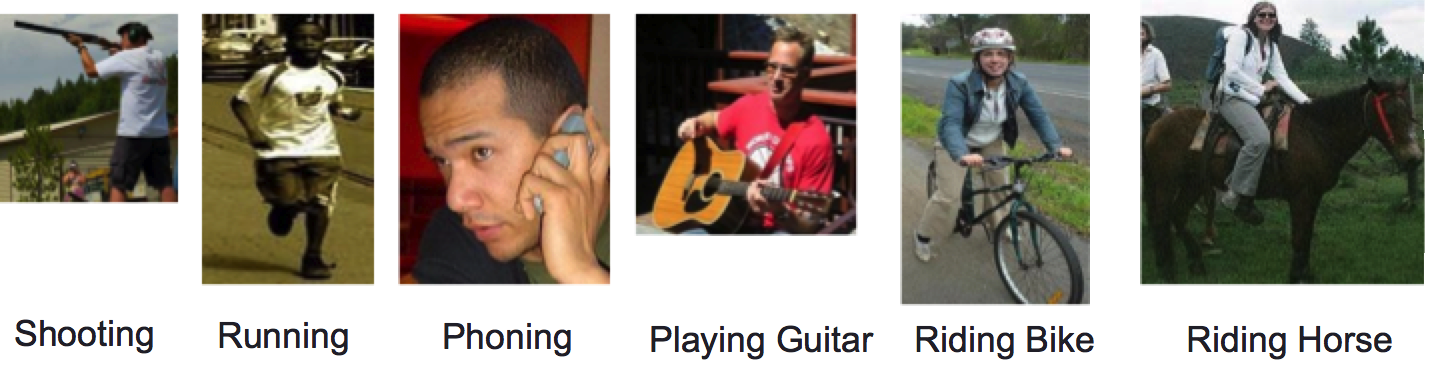
\includegraphics[width=1\textwidth]{./imageSet.png}
\caption{Samples from the image data set used in experiments \cite{li2011actions}}
\end{figure}

\subsubsection{Performance of spatial pyramid matching}
To examine the performance of spatial pyramid matching, a vocabulary with 300 was built from all SIFT features extracted from the total 360 images using Mini-Batch K-Means cluster algorithm. Next, three kinds of pyramids were built: one-level, two-level and three level. In the process of building pyramids, histograms at different levels were concatenated together to form a long vector with respective weights. As a result, one-level pyramid was a 300-dimensional vector, two-level pyramid was a 1500-dimensional vector and three-level pyramid was a 6300-dimensional vector. As for classification, SVM with 5 different kernels and KNN were employed based on different pyramid representations. In this experiment, 40 images each class were randomly chosen to act as training data while the left 20 images each class were used as testing data set. Also, the recognition accuracy is defined as 
\begin{equation}
\text{recognition accuracy} = \frac{\text{correct predictions}}{\text{number of testing samples}}
\end{equation}
where correct predictions represent the number of testing samples which are correctly predicted. The recognition results using the above settings are reported in Table 5 and 6. \\

\begin{table}[!ht]
    \begin{center}

      \begin{tabular} {cccc}
      \hline
    	\head{SVM} & \head{One-level} & \head{Two-level} & \head{Three-level}\\
      \hline
      Linear & 74.17 & 80 & {\bf 87.5} \\
      Poly & 70 & 62.5 & 31.67 \\
      RBF & 37.5 & 83.33 & 74.17 \\
      Sigmoid & 16.67 & 16.67 & 16.67 \\
      Histogram Intersection & 79.17 & 82.5 & {\bf 85} \\
      \hline
      \end{tabular}
    
    \end{center}
    \caption{Recognition accuracies (percent) of different spatial pyramids using SVM with different kernels}
\end{table}

\begin{table}[!ht]
	\begin{center}

	  \begin{tabular} {cccc}
	  \hline
		\head{} & \head{One-level} & \head{Two-level} & \head{Three-level}\\
	  \hline
      KNN & 50.83 & 45 & 48.33 \\
      \hline
      \end{tabular}
    
    \end{center}
    \caption{Recognition accuracies (percent) of different spatial pyramids using KNN}
\end{table}

\noindent Table 5 above reports the recognition accuracies using SVM with different kernels for different pyramids. The kernel types which projects samples into higher dimensional space like ``Poly'' and ``RBF'' abd ``Sigmoid'' performed much worse than ``Linear'' and ``Histogram Intersection''. Also, it is easy to see that the recognition accuracies increased by fusing information from multiple levels. For ``Linear'' and ``Histogram Intersection'', their performances were improved significantly from one-level pyramid to three-level pyramid, and ``Linear'' achieved the best result $87.5 \%$ while ``Histogram Intersection'' achieved the second best result $85 \%$ at three-level pyramid. Table 6 depicts the performance of KNN when the number of neighbors was set to 5. Compared with reasonable result of SVM, KNN did not perform quite well. The best result achieved at one-level $50.83\%$ is much smaller than $74.17\%$ which was achieved by SVM with ``Linear'' kernel. Such result makes sense because it is generally thought that KNN performs worse than SVM since KNN is a lazy learner which does not consider the global information. 

\subsubsection{Performance of earth mover's distance}
EMD was also experimented to examine its effectiveness in recognition. Following the method introduced before, each image was divided into 4 pieces equally, and EMD attempted to align these 4 pieces. In this experiment, the distance matrix calculated with EMD was referred as aligned distance while the distance matrix without EMD was referred as unaligned distance. Once distances were calculated, they were transformed into four different kernels. Finally, these kernel matrices are input into SVM for classification. Unlike previous division of training and testing samples, this experiment randomly selected $50\%$ images as training data and the other $50\%$ as testing data. The result using the above settings is recorded in Table 7. 

\begin{table}[!ht]
	\begin{center}

	  \begin{tabular} {ccccc}
	  \hline
		\head{} & \head{RBF} & \head{LAP} & \head{ID} & \head{ISD}\\
	  \hline
      Aligned Distance & 79.44 & 76.11 & 73.89 & 75.56 \\
      Unaligned Distance & 78.89 & 75.56 & 73.33 & 75 \\
      \hline
      \end{tabular}
    \end{center}

    \caption{Comparison of recognition accuracy between aligned distance and unaligned distance}
\end{table}

\noindent For all four kernel types, aligned distance performed better than unaligned distance. Though slightly, it shows the robustness of EMD which gives a more accurate image-to-image distance. Also, it is worth noting that these four kernels output different results. So it is important to select a good kernel in order to build a robust classifier. 


\subsection{Video recognition}
\subsubsection{Data set description}
The data set used in this experiment is retrieved from Visual Computing Group of Nanyang Technological University, and this data set has been used for comprehensive experiments in \cite{duan2012visual}. There are two different domains \cite{loui2007kodak}: one comes from the Kodak Consumer Video Benchmark Data set while the other comes from Youtube. Also, there are two types of features: one is SIFT while the other one is space-time feature. According to the accuracies of different feature reported in \cite{duan2012visual}, SIFT is preferred. There are six different classes, and the numbers of videos in each class from different domains are summarized in the below table.

  \begin{table}[!ht]
    \begin{center}
    
      \begin{tabular}{cccccccc}
      \hline
      \head{} & \head{Wedding} & \head{Sports} & \head{Show} & \head{Picnic} & \head{Parade} & \head{Birthday} & \head{Total}\\
      \hline
      Kodak & 27 & 75 & 57 & 6 & 14 & 16 & 195\\
      Youtube & 91 & 260 & 200 & 85 & 119 & 151 & 906\\
      \hline
      \end{tabular}
    
    \end{center}
    \caption{Number of videos in each class from Kodak and Youtube}
  \end{table}

\subsubsection{Performance of aligned space-time pyramid matching}
To examine Aligned Space-Time Pyramid Matching, a visual vocabulary is firstly needed in order to convert videos into stacks of histograms. The visual vocabulary with 2500 words was built on SIFT features sampled from features of Kodak data set. Due to a lack of memory, the size of training data was $167837 \times 128$. Although the training size was relatively small, fortunately, it still produced comparable results compared with performances reported in \cite{duan2012visual}. The next step was to convert all Kodak videos into either one stack of histograms (level 0) or 8 stacks of histograms (level 1) based on the visual vocabulary built before. Once Bow models for all Kodak videos are built, EMD was employed to calculated video-to-video distances among all these videos. In this experiment, the C program wrote by Rubner, who is the proposer of Earth Mover's distance \cite{rubner2000earth}, was used. To integrate this C program with the main codes written in Python, an interface was added to enable communications between these two modules. Please also note that the time taken by calculating level one distances is around 65 times of that taken by calculating level 0 distance. When calculating level one distance, the number of pairwise distances needed is $8 \times 8 = 64$. If the aligned process is also considered, the number of times to invoke EMD becomes 65. However, for level 0 distance, only one time is needed to call EMD when calculating the distance between two videos. Similar to the settings in image recognition, distances were then transformed into kernels using Gaussian, Laplacian, ISD and ID. The final step was to employ SVM to perform recognition based on these gram matrices. Due to the poor performance of KNN, KNN was not tried here. Furthermore, a new mode fusing SVM scores from Gaussian, Laplacian, ISD and ID was tried, and this fusing process is defined as
\begin{equation}
f^{Fuse} = \frac{1}{N} \sum_{i=1}^{N} \frac{1}{1 +\exp{(-f_i)}}
\end{equation}

\noindent where $N$ is the number of classifiers, and $f_i$ is the score output by $i$th classifier. In this case, $N = 4$, and the four SVM classifiers were built from Gaussain, Laplacian, ISD and ID kernel matrices. \\

\begin{table}[!ht]
  \begin{center}
  \scalebox{0.9}{
    \begin{tabular} {cccccc}
    \hline
    \head{} & \head{Gaussian} & \head{Laplacian} & \head{ISD} & \head{ID} &\head{Fused scores}\\
    \hline
    Level 0 & $44.38 \pm 2.13$ & $44.90 \pm 2.73$ & $44.01 \pm 2.13$ & $45.36 \pm 3.13$ & $44.33 \pm 2.61$ \\
    Level 1 (Unaligned) &$43.08 \pm 3.14$ &$43.85\pm3.84$ &$43.22\pm3.11$ &$43.85\pm3.56$ &$43.55\pm3.46$ \\
    Level 1 (Aligned)&$43.61\pm2.97$ &$43.40\pm3.18$ &$43.46\pm2.97$ &$43.22\pm3.11$ & $44.08\pm3.25$ \\
      \hline
      \end{tabular}
      }
    \end{center}
    \caption{Means and standard deviations (percent) of MAPs over six events at different levels using SVM with different kernels.}
\end{table}

\noindent In the experiment shown in Table 9, each time three videos from each class were selected as training data while the rest of Kodak videos were used as testing videos. As a result, 18 videos were used to train models while the rest 177 videos acted as testing videos. Furthermore, SVM was trained in one-against-all manner, which trains in total 6 classifiers for all 6 events. This experiment was repeated for five times, and the mean and standard deviation of Mean Average Precision (MAP) for each method was recorded in Table 9. Given the fact that only around $9.23\% \; (\sfrac{18}{195})$ videos were used as training data, the performance reported in Table 9 was quite good. There are three observations based on results in Table 9. 
\begin{enumerate}
  \item{\bf In this case, Level 0 performs better than both unaligned Level 1 and aligned Lavel 1 for all types of kernel} \\
  The most possible reason is due to a lack of training data. In latter experiments, when all youtube videos and randomly selected 18 Kodak videos were used for training, the performance ranking was: Level 1 (Aligned) $>$ Level 1 (Unaligned) $>$ Level 0. 

  \item{\bf Level 1 (Aligned) performed better than Level 1 (Unaligned) in most cases}\\
  Thus, the one additional alignment makes worthwhile contribution to a better performance though it requires one more call of EMD. 

  \item{\bf The approach of fusing scores provides a guarantee on performance}\\
  For all three cases, the means of MAP using fused scores were always not the worst, and it was even the best for aligned Level 1 distance. Therefore, it provides a good insight that fusing scores of multiple classifiers is a good alternative if the standalone performances of those classifiers are unclear.

\end{enumerate}

\begin{table}[!ht]
  \begin{center}
  \scalebox{0.9}{
    \begin{tabular} {cccccc}
    \hline
    \head{} & \head{Gaussian} & \head{Laplacian} & \head{ISD} & \head{ID} &\head{Fused scores}\\
    \hline
     bxx& $40.20 \pm 2.57$ & $38.35 \pm 2.31$ & $39.93 \pm 2.58$ & $38.23 \pm 2.08$ & $39.34 \pm 2.55$ \\
     txx& $44.28 \pm 2.14$ & $44.90 \pm 2.73$ & $44.01 \pm 2.13 $ & $45.36 \pm 3.13 $ & $44.33 \pm 2.61$ \\
     txc& $ 42.15 \pm 4.73$ & $45.01 \pm 3.45$ & $43.47 \pm 4.56$ & $45.38 \pm 3.20$ & $44.11 \pm 3.90$ \\
     tfx& $ 43.76 \pm 2.99$ & $44.14 \pm 3.36$ & $43.61 \pm 3.03$ & $44.05 \pm 3.51$ & $44.18 \pm 3.22$ \\

     tfc& $ 43.71\pm 1.37$ & $\mathbf{46.02 \pm 1.84}$ & $\mathbf{44.93 \pm 1.64}$ & $\mathbf{46.21 \pm 1.83}$ & $\mathbf{45.28 \pm 1.62}$ \\
     Easy soft& $43.54 \pm 2.12$ & $ 44.77\pm 2.41$ & $43.52 \pm 2.08$ & $45.24 \pm 2.47$ & $ 44.79\pm 2.55$ \\
     Gaussian soft& $\mathbf{44.77 \pm 2.80}$ & $45.23 \pm 2.76$ & $44.90 \pm 3.01$ & $45.23 \pm 2.87$ & $\mathbf{45.20 \pm 3.04}$ \\
      \hline
      \end{tabular}
      }
    \end{center}
    \caption{Means and standard deviations (percent) of MAPs over six events using different mechanisms to build histograms}
\end{table}

\noindent Experiments on building better BoW using different weighting schemes and soft assignment were also tried. Following the same setting of experiments in Table 9, the results of various approaches were recorded in Table 10. ``Easy soft'' represents the approach that the top $T$ neighbors are retrieved for each feature when building histograms. In this experiment, $T = 4$. ``Gaussian soft'' represents the approach which uses Gaussian Mixture Models to build histograms. For other approaches like ``txc'', please refer to Table 4 in the section of representations of videos. Based on results shown in Table 10, it is not easy to that ``tfc'' and ``Gaussian soft assignment'' performs relatively better than the rest approaches. Thus, histograms built through soft assignment and weighting schemes which consider global frequencies of visual words possess more discriminable power. \\

\begin{table}[!ht]
  \begin{center}

    \begin{tabular} {cccc}
    \hline
    \head{Training videos} & \head{Testing videos} &\head{Original videos} &\head{Compressed videos}\\
    \hline
    60 & 846 &  $38.9 \pm 2.9$  & $38.6 \pm 2.8$ \\
    120 & 786 & $45.7 \pm 2.2$  & $44.5 \pm 1.6$ \\
    180 & 726 & $49.5 \pm 1.8$  & $48.3 \pm 1.9$ \\
    240 & 666 & $52.0 \pm 2.1$  & $50.6 \pm 2.1$\\
    \hline
    \end{tabular}

    \end{center}
    \caption{Recognition accuracies (percent) using distances calculated on original Youtube videos and distances calculated on Youtube compressed videos.}
\end{table}
\noindent The approach of identifying key frames in a cluster of images introduced in the section of image recognition was employed to compress Youtube videos. Originally, the total size of Youtube histograms in Python serialization file was 4.42 GB. After compressing, the size was reduced to 3.17 GB, which means around $28.41 \%$ frames were discarded. Then the level 0 distance matrix of compressed Youtube videos using Aligned Space-Time Pyramid Matching was calculated. In this experiment, SVM was trained in one-against-one manner to recognize multiple classes. The distance of original Youtube videos were used as a baseline to compare the performance of compressed videos. Table 11 depicts the recognition accuracies for these two distance matrices using different number of training videos. There are two observations based on Table 11.
\begin{enumerate}
  \item{\bf The performance of compressed videos is slightly worse than original videos} \\
  Though compressed videos contain less redundant frames, the performance is still worse than original videos. The most possible explanation is that EMD always finds the best matches among frames. Thus, those redundant frames are actually ignored during the calculation of distances. As a result, it shows the effectiveness of EMD. 

  \item{\bf With more training samples, the recognition accuracy increases}
  This is actually common sense. With more training samples, the found boundary is more likely to be near to the optimal bounday. However, the problem is there is normally no enough labelled samples. This is also the main reason why researchers are exploring domain adaptations. 
\end{enumerate}

\subsubsection{Performance of specialized GMM}
\begin{table}[!ht]
  \begin{center}
  \scalebox{0.9}{
    \begin{tabular} {cccccc}
    \hline
    \head{} & \head{Gaussian} & \head{Laplacian} & \head{ISD} & \head{ID} &\head{Fused scores}\\
    \hline
    spherical 128& $24.70 \pm 1.41 $ & $ 43.04 \pm 1.61 $ & $26.92 \pm 1.00$ & $\mathbf{43.64 \pm 0.96}$ & $ 32.91 \pm 2.20$ \\
    spherical 64& $ 23.99 \pm 1.40$ & $42.35 \pm 1.64$ & $ 25.62\pm 1.11$ & $43.42 \pm 1.18$ & $29.01 \pm 1.10$ \\
    full 128& $ 25.69 \pm 7.57 $ & $21.39 \pm 7.32$ & $26.49 \pm 8.38$ & $21.93 \pm 7.75$ & $21.79 \pm 7.29$ \\
    full 64& $  25.23 \pm 0.94$ & $ 29.69 \pm 1.81$ & $25.68 \pm 1.34$ & $30.74 \pm 1.67$ & $26.74 \pm 1.63$ \\
    \hline
    \end{tabular}
    }
    \end{center}
    \caption{Means and standard deviations (percent) of MAPs over six events using different GMMs}
\end{table}
\noindent Experiments using another representations of video clips are presented here. There are in total four different settings controlled by the type covariance and the dimension of SIFT feature. Two types of covariances were adopted in experiments: spherical and full. While spherical covariance assumes that the variations on all dimensions are the same, full covariance does not have such assumption. An example to demonstrate the differences of these two types of covariances is Figure 14, where spherical covariance builds Gaussian distributions in circle shape, and full covariance builds in ellipse. Also, the dimension of SIFT was reduced to 64 through PCA for experiments. \\ 

\begin{figure}[!ht]
\centering
  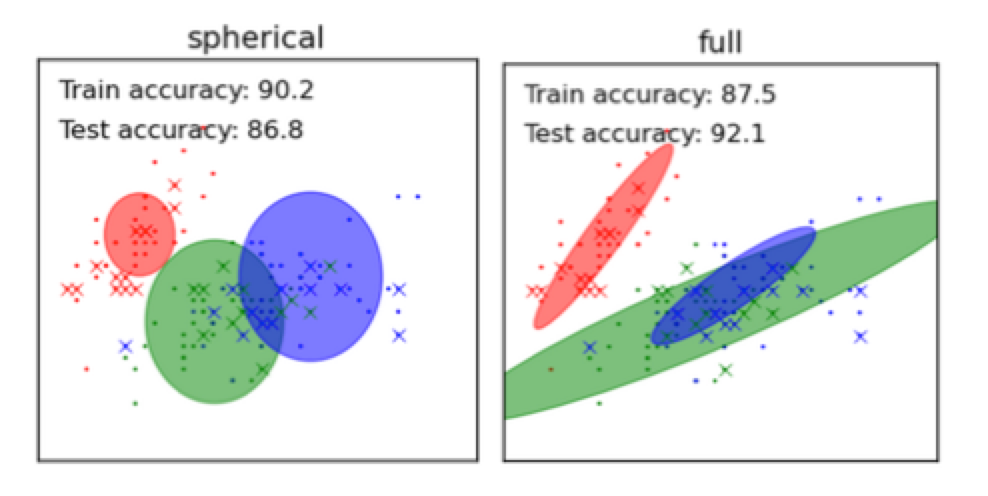
\includegraphics[scale = 0.6]{./DifCov.png}
\caption{Gaussian Mixtures Models built by different covariance types \cite{scikit-learn}.}
\end{figure}

\noindent Based on results in Table 12, there are two observations. 
\begin{enumerate}
  \item{\bf Spherical covariance performed better than full covariance}\\
  Except for Gaussian kernel, the performances of spherical covariance with 128 dimensional SIFT features were better than those of full covariance. The possible reason could be that the number of features was not enough to build good enough specialized GMM for most video clips when full covariance was adopted. 

  \item{\bf Spherical covariance using ID kernel performed the best}\\
  Overall speaking, GMM representations of videos did not perform well compared with Bow representations. However, the best MAP achieved by spherical covariance using 128 dimensional feature reached $43.64 \%$, which is slightly worse than that achieved by level 0 distance using aligned space-time pyramid matching. This gives an insight that a right kernel type helps a lot to improve the performance. 
\end{enumerate}


\subsubsection{Performance of concept attributes}
\begin{table}[!ht]
  \begin{center}

    \begin{tabular} {cc}
    \hline
    \head{} & \head{Recognition accuracy}\\
    \hline
    Kodak $\to$ Kodak & $38.5 \pm 12.7$\\
    Youtube $\to$ Kodak & $30.0 \pm 6.9$\\
    Baseline & $41.6 \pm 11.5$\\
    \hline
    \end{tabular}

    \end{center}
    \caption{Means and standard deviations (percent) of recognition accuracies using concept attributes}
\end{table}
\noindent Concept attribute was also experimented. In this experiment, 2-layer SVM classification structure was implemented, where the first layer built up 6 concept detectors, and the second layer trained and tested videos using 6-dimensional vectors, in which each dimension represented the respective semantic concept like ``birthday'' and ``show''. The results were presented in Table 13. ``Kodak $\to$ Kodak'' represents the case where training samples in Kodak videos were used to train concept detectors, whereas ``Youtbe $\to$ Kodak'' represents the case where all Youtube videos were used to train concept detectors. The second stage SVM was implemented in one-against-one manner with Gaussian kernel. Baseline was implemented using the average kernel generated from 4 types of kernel matrix. Based on results recorded in Table 13, there are two observations.
\begin{enumerate}
  \item{\bf ``Youtbe $\to$ Kodak'' performed much worse than ``Kodak $\to$ Kodak''}\\ This result makes sense since Youtbe videos and Kodak videos come from two different domains. Therefore, their distributions are quite different. 

  \item{\bf ``Kodak $\to$ Kodak'' was slightly worse than baseline}\\
  This observation demonstrates the promising discriminable power of concept attribute. Though the representation of videos is reduced into 6-dimensional vectors, its performance is still comparable with that by basline. Actually, concept attribute could be implemented to perform better by adding more concepts. However, there was no enough training data. 

\end{enumerate}


\subsubsection{Performance of domain adaptation methods}
This subsection introduces the experiments on domain adaptation methods. There are in total four domain adaptations: Feature Replication (FR), Adaptive SVM (A-SVM), Domain Transfer SVM (DTSVM) and Adaptive Multiple Kernel Learning (A-MKL). The other three methods SVM\_T, SVM\_AT and MKL are used as baseline, where SVM\_T only relied on $\mathcal{D}_l^T$, and SVM\_AT relied on training samples from both $\mathcal{D}^T$ and $\mathcal{D}^A$, and MKL used the average of all kernel matrices. Therefore, except SVM\_T, all other 6 methods needed all Youtube videos as training data in $\mathcal{D}^A$. In Table 14, various distance matrices are listed which have been implemented. Once a distance matrix was given, 20 kernel matrices were built, where Gaussian, Laplacian, ISD and ID were employed by setting kernel parameter as $\gamma = 2^l \gamma_0$, and $l \in (-3, -2,\cdots, 1)$. Such setting was made to align with that stated in \cite{duan2012visual}. One special case was MAP(8) in which 2 different distance matrices were input. As a result, there were in total 40 base kernels for MAP(8) during the process of all these methods. As for the division of training samples and testing samples, each time the experiment randomly selected 3 videos from Kodak set as $\mathcal{D}_l^T$ while the left videos were treated as $\mathcal{D}_u^T$. All Youtube videos were used as full labelled set in $\mathcal{D}^A$ if needed. The results of repeating this experiment for five times were recorded in Table 15 as below.\\

\begin{table}[!ht]
  \begin{center}
  \scalebox{0.9}{
    \begin{tabular} {cl}
    \hline
    \head{Setting Name} & \head{Content}\\
    \hline
    MAP(1) & Level 0 distance in aligned space-time pyramid matching \\
    MAP(2) & unaligned Level 1 distance in aligned space-time pyramid matching \\
    MAP(3) & aligned Level 1 distance in aligned space-time pyramid matching \\
    MAP(4) & distances calculated by histograms built in ``tfc'' weighting scheme \\
    MAP(5) & distances calculated by histograms built by straightforward soft assignment \\
    MAP(6) & distances calculated by histograms built by GMM soft assignment \\
    MAP(7) & \vtop{\hbox{\strut distances calculated by specialized GMMs built on 128 dimensional SIFT} \hbox{\strut features with spherical covariance}} \\
    MAP(8) & \vtop{\hbox{\strut two set of distances: aligned Level 1 distances and distances from histograms} \hbox{\strut built through GMM soft assignment}} \\

    \hline
    \end{tabular}
  }
    \end{center}
    \caption{Experimental settings}
\end{table}


\begin{table}[!ht]
  \begin{center}
  \scalebox{0.8}{
    \begin{tabular} {cccccccc}
    \hline
    \head{} &\head{SVM\textunderscore T} &\head{SVM\textunderscore AT} &\head{FR} &\head{A-SVM} &\head{MKL} &\head{DTSVM} &\head{A-MKL} \\
    \hline
    MAP(1) & $44.33 \pm 2.61$ & $52.21 \pm2.54$ & $52.33 \pm 2.20$ & $47.03 \pm3.26$ & $50.82 \pm2.16$ & $47.14 \pm3.26$ & $54.29 \pm 2.21$ \\

    MAP(2) & $43.55 \pm3.46$&  $55.37 \pm2.26$&  $55.95 \pm 3.79$  &$45.86 \pm4.39$ & $55.08 \pm 6.17$  &$50.97 \pm 1.38$ & $54.26 \pm 3.46$ \\
    MAP(3) & $44.08 \pm 3.25$ & $57.56 \pm3.02$ & $53.91 \pm 1.48$ & $45.42 \pm 3.62$ &$53.81 \pm 3.86$ & $53.32 \pm 2.56$ & $\mathbf{57.45 \pm 1.64}$ \\

    MAP(4) &
    $ 45.27 \pm 1.63$ & $ 51.83 \pm 2.27$ & $52.55 \pm 2.00$ & $45.94 \pm 1.70 $ & $51.70  \pm 2.35$ & $52.31  \pm 2.56$ & $53.05\pm 2.21$ \\

    MAP(5) & 
    $44.79 \pm 2.55$ & $47.80 \pm 1.67$ & $51.89 \pm 1.99$ & $47.41 \pm 3.13$ & $47.16 \pm 1.77$ & $45.05 \pm 4.07$ & $51.08 \pm 2.87$ \\

    MAP(6) &
    $45.20 \pm 3.04$ & $56.90 \pm 2.79$ & $54.03\pm 4.02$ & $46.62 \pm 3.14 $ & $55.47 \pm 4.11$ & $53.41 \pm 3.29$ & $\mathbf{59.16 \pm 3.38}$ \\

    MAP(7) &
    $32.91 \pm 2.20$ & $33.15 \pm 1.78$ & $41.78 \pm 3.98 $ &$37.07 \pm 3.52$  &$33.64 \pm 0.74$ & $\mathbf{46.61 \pm 2.41}$ & $35.88 \pm 1.98$ \\

    % Voc1000 Level 0 &
    % $ 44.23 \pm 3.20 $ & $53.67 \pm 3.29$ & $52.16 \pm 4.00$ & $45.07 \pm 4.05$ & $52.33 \pm 4.23$ & $49.90 \pm 3.47$ & $ 55.99\pm 3.79$ \\

    MAP(8) &
    $ 44.69\pm 2.84$ & $ 60.21 \pm 1.94 $ & $55.29 \pm 3.00$ & $46.28 \pm 4.23 $ & $ 58.36 \pm 3.75$ & $ 57.01 \pm 2.45 $ & $\mathbf{61.40 \pm 1.91}$ \\

    % Aligned L1 + Gau Ass + Voc1000 L0 &
    % $44.92 \pm 2.92$ & $58.80 \pm 2.68$ & $ 54.15 \pm 3.20 $ & $45.76 \pm 4.10$ & $56.82 \pm 4.00$ & $56.52 \pm 2.70$ & $59.83 \pm .82$ \\
    \hline
    \end{tabular}
    }
    \end{center}
    \caption{Means and standard deviations (percent) of MAPs over six events for all methods}
\end{table}

\noindent Table 15 gives the means and standard deviations of MAPs over six events for all methods, and there are 4 observations.
\begin{enumerate}
  \item{\bf In all cases, SVM\_AT performed better than SVM\_T}\\
  This result is in expectation, and it demonstrates the limitation of classifiers built from limited training samples in $\mathcal{D}^T$. If there are more labelled samples from $\mathcal{D}^A$ used in training, the resulting classifiers are generally more robust. 

  \item{\bf Over almost all 7 methods from SVM\_T to A-MKL, the distance matrix calculating from histograms built by Gaussian soft assignment(MAP(6)) performed better than other 6 distance matrices from MAP(1) to MAP(5) and MAP(7)}\\
  This statement is made without considering MAP(8) which used 2 kinds of distance matrices. This result strongly shows the robustness of histograms built through Gaussian soft assignment. During the process of building histograms through Gaussian soft assignment, more discriminable power is retained compared with other approaches. 

  \item{\bf A-MKL performed the best}\\
  MAP(8) achieved the best using A-MKL, where aligned Level one distance and distance from Gaussian soft assignment were used. A-MKL utilizes information from pre-learnt classifiers and reduces the mismatch between $\mathcal{D}^T$ and $\mathcal{D}^A$ by finding the optimal coefficients of multiple base kernels. Though there are at least $20\%$ noisy labels in Youtube videos as reported in \cite{duan2012visual}, A-MKL still learned a robust classifier and achieved the best. The best MAP $61.40\%$ is better than the results reported in \cite{duan2012visual}, and it demonstrates the effectiveness of selecting base kernels smartly. 

  \item{\bf DTSVM performed amazingly in MAP(7)}\\
  In MAP(7), the distance matrix from specialized GMMs were used for experiments. Normally, its performance was less than $38\%$ indicating that many specialized GMMs were not well built. However, DTSVM helped to increase the performance from the lowest $32.91\%$ to $46.61\%$. This result strongly shows the importance of exploring the optimal coefficients for base kernels.

\end{enumerate}
